\documentclass[11pt]{article}

\usepackage[utf8]{inputenc} % Required for inputting international characters
\usepackage[T1]{fontenc} % Output font encoding for international characters
\usepackage{circuitikz}
\usepackage[portuguese]{babel}
%\usepackage[margin=10mm]{geometry}
\usepackage{mathpazo} % Palatino font
\usepackage{graphicx}
\usepackage{pgfplots}
\usepackage[margin=20mm]{geometry}
\graphicspath{{/home/hiago/Desktop/}}
\usepackage{hyperref}
\begin{document}

%----------------------------------------------------------------------------------------
%	TITLE PAGE
%----------------------------------------------------------------------------------------

\begin{titlepage} % Suppresses displaying the page number on the title page and the subsequent page counts as page 1
	\newcommand{\HRule}{\rule{\linewidth}{0.5mm}} % Defines a new command for horizontal lines, change thickness here
	
	\center % Centre everything on the page
	
	%------------------------------------------------
	%	Headings
	%------------------------------------------------
	
	\textsc{\LARGE Relatório da XIII Jornada
de Iniciação Científica e Tecnológica}\\[1.5cm] % Main heading such as the name of your university/college
	
	\textsc{\Large Bolsa PIBIC/LNCC}\\[0.5cm] % Major heading such as course name
	
	%\textsc{\large Relatório da sexta experiência}\\[0.5cm] % Minor heading such as course title
	
	%------------------------------------------------
	%	Title
	%------------------------------------------------
	
	\HRule\\[0.4cm]
	
	{\huge\bfseries  Localização de Robôs Móveis via Filtro de Kalman}\\[0.4cm] % Title of your document
	
	\HRule\\[1.5cm]
	
	%------------------------------------------------
	%	Author(s)
	%------------------------------------------------
	\begin{flushleft}
	

			\large
			\textit{Bolsista: } 
			Hiago Riba Guedes % Your name
						\large \\
			\textit{Orientador: }
			Marcelo Dutra Fragoso % Supervisor's name\\
			\\ \textit{Período: } 01/08/2017 a 31/07/2018  	\\

			\textit{Projeto: } 800333/2016-0

		\end{flushleft}
	% If you don't want a supervisor, uncomment the two lines below and comment the code above
	%{\large\textit{Author}}\\
	%John \textsc{Smith} % Your name
	
	%------------------------------------------------
	%	Date
	%------------------------------------------------
	
	\vfill\vfill\vfill % Position the date 3/4 down the remaining page
	Petrópolis\\
	{\large\today} % Date, change the \today to a set date if you want to be precise
	
	%------------------------------------------------
	%	Logo
	%------------------------------------------------
	
	%\vfill\vfill
	%\includegraphics[width=0.2\textwidth]{placeholder.jpg}\\[1cm] % Include a department/university logo - this will require the graphicx package
	 
	%----------------------------------------------------------------------------------------
	
	\vfill % Push the date up 1/4 of the remaining page
	
\end{titlepage}
\newpage

%\tableofcontents
\newpage
\section{Objetivos}
Este trabalho tem como objetivos a confecção de um robô móvel e a aplicação do Filtro de Kalman a fim de eliminar os ruídos existentes na sua aquisição de dados. \\

Na qual podemos categorizar da seguinte maneira:
\begin{itemize}
\item Adquirir os componentes e realizar sua montagem
\item Estudar e aplicar os filtros de Kalman
\item Aplicar os dados a um controle PID
\end{itemize}
\section{Introdução}
O robô terá inteligência simples ,sendo de competência  própria apenas o desvio de obstáculos e ele deverá nos fornecer em que ponto do mapa ele se encontra em relação ao seu ponto de origem. E via Bluetooth nos oferecer suas coordenadas locais.
\section{Materiais e Métodos }

Seguindo os passos estipulados pelo objetivo temos:

\subsection{Montagem do Robô}
 Para a confecção do hardware do robô foram utilizados dois microcontroladores com arquitetura AVR,onde a eles confere o objetivo de adquirir os dados dos sensores presentes , tais como sensores de velocidade ,giroscópio e ultrassom e fazer a sua devida filtragem com o objetivo final de ter conhecimento da sua localização ótima. 4 Baterias do tipo 18650 foram utilizados a fim de termos uma tensão de alimentação próxima aos 15 V,suficientes para dar uma autonomia razoável para o mesmo, contamos também com uma placa responsável para a proteção e carregamento adequado das baterias.

 
 \begin{center}
 \begin{figure}[!h]
 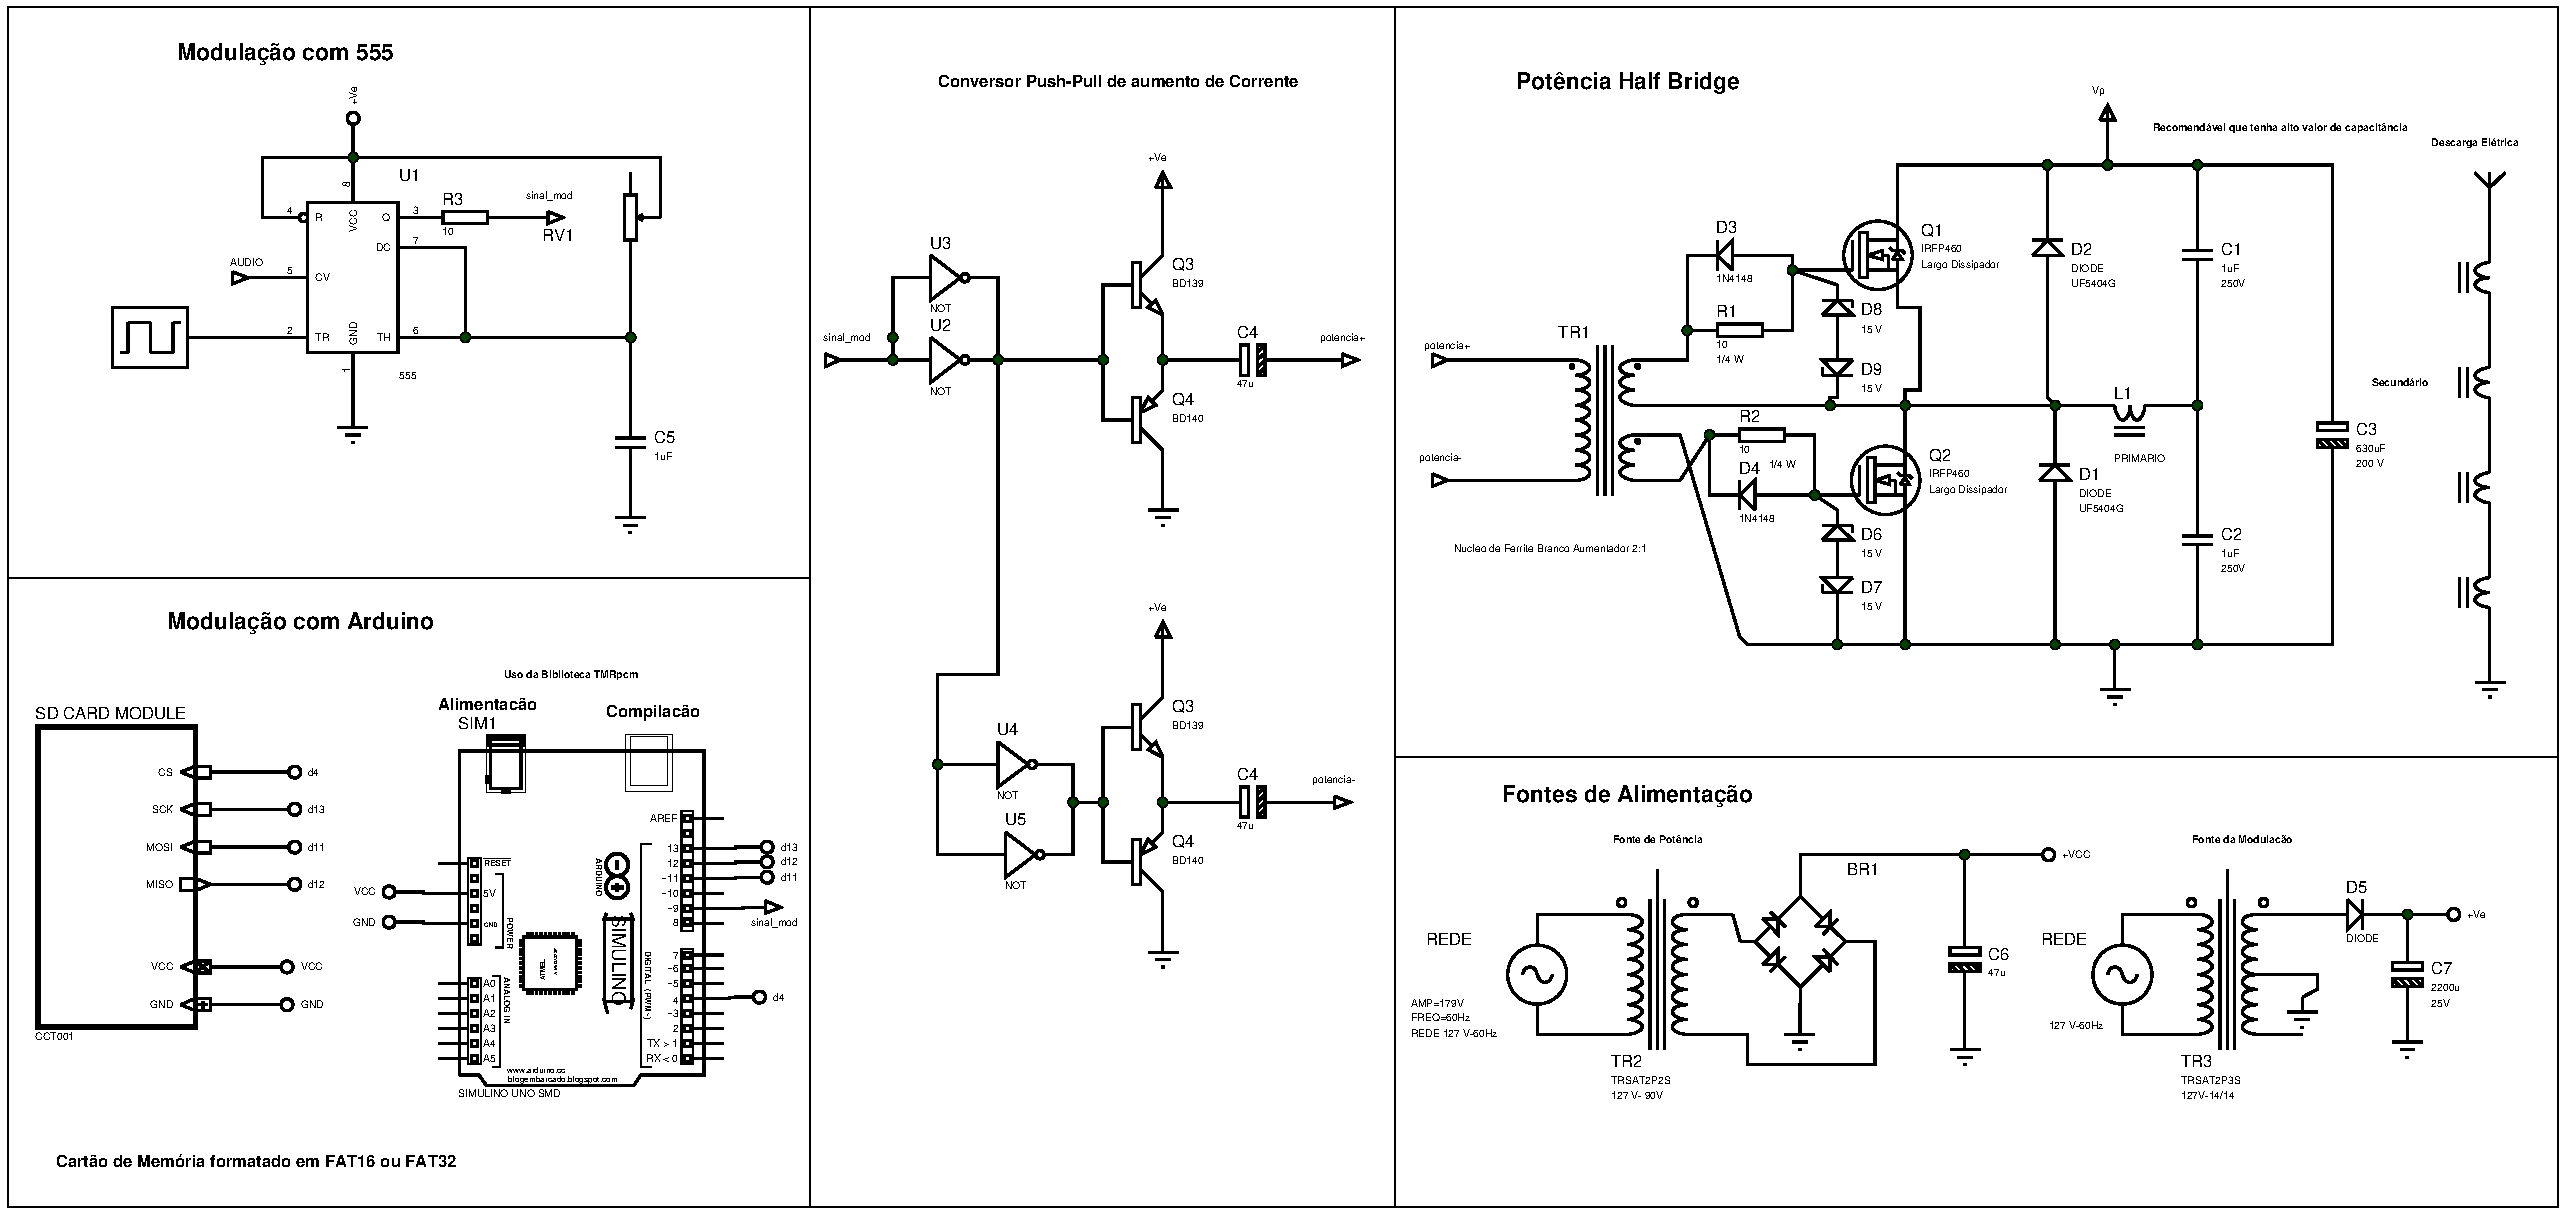
\includegraphics[scale=0.5]{esquematico.pdf}
 \caption{Esquemático(provisório) do hardware do Robô} 
 \end{figure}
 \end{center}

\subsection{O Filtro de Kalman}
Conhecido por ser um dos muitos responsáveis por levar o homem a Lua no projeto Apollo o Filtro de Kalman se mostra bastante usual nos dias de hoje com os carros autônomos. Por ser  um algoritmo recursivo e por atuar no erro médio quadrado esse filtro se mostra bastante prático para resolver o problema de ruído que ocorre no sensoriamento.

 Equação de predição de estado a priori\\
$$
\hat{x_{k}}^{-}=A\hat{x}_{k-1}^{+} +Bu_k $$
$$
P_{k}^{-}=AP_{k-1}^{+}A^{T} + C_kQC_k^T
$$

Agora mostrando as equações a posteriori\\

$$
\hat{x}_{k}^{+}=\hat{x_{k}}^{-} + K_{k}(z_{k} - H\hat{x}_k^-)
$$
$$
P_{k}^{+}=P_k^- -K_kH_kP_k^- 
$$
$$
K_k=P_k^{-}H^{T}_{k}(H_k P_{k}^{-}H_k^{T}+R_{k})^{-1}$$


 Onde entraremos com nossos parâmetros pertinentes na entrada, que seriam as coordenadas dadas pelos nossos sensores (que no caso são as coordenadas x,y e a orientação $\theta$ )
 \subsection{Os Modelos Utilizados}
 Foram utilizados dois modelos para conseguirmos estudar o filtro de Kalman no robô móvel, o modelo linear que nessa aplicação é chamado de Modelo Cinemático e o modelo Não-Linear que também é chamado de modelo Dinâmico.
 \subsubsection{Determinação das Matrizes no sistema Cinemático}
 $$
A_k=\left[\begin{array}{ccc}
 x_k&0 &\Delta s \cos(\theta + \frac{\Delta \theta}{2}) \\
 0&y_k &\Delta s \sin(\theta + \frac{\Delta \theta}{2}) \\
 0&0&\theta_0 +\frac{\Delta \theta}{2}
\end{array}\right]
$$
Como o robô terá uma inteligência um tanto rudimentar como não bater em nenhuma parede , a matriz de modelo das medidas será a matriz identidade dos estados.
$$H_k=
\left[
\begin{array}{ccc}
1 & 0 & 0\\
0 & 1 & 0\\
0 & 0 & 1
\end{array}
\right]
$$
\subsubsection{Determinação da Matriz no sistema Dinâmico}
$$
A_k=\left[
\begin{array}{ccc}
1 & 0 & -\dot{\theta}_l\frac{r}{2}sin(\theta_{t-1})-\dot{\theta}_r\frac{r}{2}sin(\theta_{t-1})           \\
0 & 1 & \dot{\theta}_l\frac{r}{2}cos(\theta_{t-1})-\dot{\theta}_r\frac{r}{2}cos(\theta_{t-1})                     \\
0 & 0 & 1
\end{array}
\right]
$$
\section{Resultados}
  \begin{center}
 \begin{figure}[!h]
 \includegraphics[scale=0.1]{roboto}
 \caption{Foto do Robô montado} 
 \end{figure}
 \end{center}

Para averiguar a eficácia dos modelos encontrados foram realizados dois testes, um teste que é utilizado pela DARPA para premiar o carro autônomo mais preciso é o de fazer com que o carro de uma volta completa em um circuito de distância conhecida e pare exatamente no mesmo local em que parou , o carro que apresentar menor erro real é considerado o vencedor. Faremos aqui uma versão mais simples porém com a mesma ideia , esticamos uma fita isolante no chão e medimos  o comprimento total dessa fita. Faremos com que o robô ande essa distância sem e com o Filtro de Kalman em seu código. Após esse teste faremos com que o robô nos dê medidas em um ambiente fechado ,da mesma forma esse teste será feito com e sem o Filtro de Kalman, esse segundo teste tem como objetivo de averiguar a inteligência do robô frente aos resultados de sua localização.
\begin{thebibliography}{9}
\bibitem{ekf} 
Robot Localization and Kalman Filters \textit{On finding your position in a noisy world}, Rudy Negenborn,
UTRECHT UNIVERSITY
Link: \url{http://www.negenborn.net/kal_loc/thesis.pdf}
\bibitem{DandV}
Stochastic Modelling and Control,
M. H. A. DAVIS and R. B. VINTER,
ISBN-13: 978-94-010-8640-0
\bibitem{IntaRob}
Introdução à Robótica,
Maja J. Mataric,
ISBN: 978-85-393-0490-5
\end{thebibliography}
\end{document}